\subsection{Cylindrical Drift Chamber - CDC}

\begin{figure}[htbp]
  \centering
  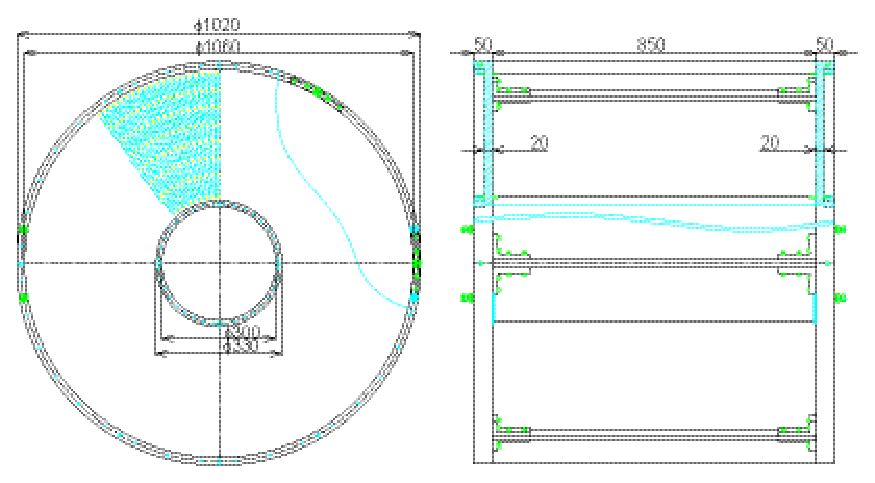
\includegraphics[width=10cm]{pic/experiment/CDC_structure.eps}
  \caption{
    Design of the CDC (all dimensions in mm).
    The CDC consists of two aluminum end-plates, a 1mm thick CFRP cylinder as an inner wall, and six aluminum posts that are placed outside the tracking volume.
  }
  \label{fig:CDC_structure}
\end{figure}

\begin{figure}[htbp]
  \centering
  \includegraphics[width=7cm]{pic/experiment/CDC_cell.eps}
  \caption{
    Cell structure of the CDC.
  }
  \label{fig:CDC_cell}
\end{figure}


The CDC is a cylindrical wire drift chamber that contains 15 layers of anode wires.
The structure of the CDC is shown in Fig\ref{fig:CDC_structure}.
The outer radius is 530mm and the inner radius is 150mm, with a total length of 950mm.
The wire length of axial layers is 833.8mm, thus the angular coverage is $49^{\circ}<\theta<131^{\circ}$ in the polar angle region corresponding to a solid angle coverage of $66\%$ of $4\pi$.
The CDC consists of two aluminum end-plates of 20mm thickness, a 1mm thick CFRP cylinder as the inner wall of the CDC, and six aluminum posts that are placed outside the tracking volume.
The CDC uses gold-plated tungsten of 30$\mu$m $\phi$ for the sense wires, and gold-plated aluminum of 100$\mu$m $\phi$ for the field and guard wires.
These wires are supported by feedthroughts with a bushing inserted at the end.
Bushes with an 80 and 200$\mu$m $\phi$ hole are used for the sense and field/guard wires, respectively.

\input{experimental/table/CDC_config}

The CDC has 15 layers of small hexagonal cells with a typical drift length of 9mm, which are grouped int 7 super layers as shown in Fig\ref{fig:CDC_cell}.
Table \ref{tab:CDC_cell} gives the detailed parameter of the wire configuration. The layers are in the radial region from 190.5mm (layer 1) to 484.5mm (layer 15).
The 8 stereo layers tilted by about 3.5$^{\circ}$ are used to obtain longitudinal position information.
The number of readout channels is 1816 and the total number of wires in the CDC is 8064.

The drift gas is 1 atm of mixed argon (50\%)-ethane (50\%). A high voltage is applied to the field and guard wires, and the sense wires are kept at ground potential.
For the first super-layer (A1) and the second one (U1), a high voltage of -2.8kV is applied to the potential wires, and -2.7kV to the potential wires of the other super-layers.
Also, -1.5kV, -1.8kV, and -0.6kV are applied to the innermost, the outermost, and the other guard wires, respectively.
